
\documentclass[12pt,a4paper,sans]{article}
\usepackage[margin=0.5in]{geometry}
\usepackage[utf8]{inputenc}
\usepackage{graphicx}
\usepackage{wrapfig}
\graphicspath{ }
\usepackage{hyperref}
\title{First document}
\usepackage[noframe]{showframe}
\author{Hubert Farnsworth \thanks{funded by the ShareLaTeX team}}
\date{February 2014}
\begin{document}
 	\begin{center}
 		 	\textbf{ANKIT KUMAR}
 		 	\\*
 			\line(1,0){250}
 		 	 	
 	\end{center}
 
 
 \begin{wrapfigure}{r}{0.25\textwidth}
	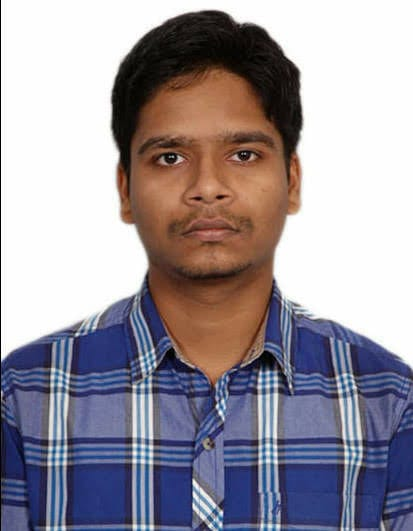
\includegraphics[width=0.15\textwidth]{pic}
 \end{wrapfigure}
Bangalore,India
\\*
Contact: 9958285598
\\*
e-mail id:ankit.tikna92@gmail.com
\\*
linked in :linkedin.com/in/akamaestro
\\* git-hub :https://github.com/AKAmaestro
\bigskip
\bigskip\bigskip\bigskip
\section*{OBJECTIVE}
Interest in developing, designing and implementing customized solutions to various tasks .Domains where one can integrate machines & humans together.Interested in working on projects involving machine learning , data analytics, and image processing + robotics as major area of interest.\\*

\section*{EDUCATION}
 
 
 \begin{tabular}{|c | c|c|c|c|}
 	
 	\hline
 	
 	\textbf{ Degree } & \textbf{   School/College   } & \textbf {  University }                                                                & \textbf{ Passing Year } & \textbf{ Percentage/CGPA } \\ \hline
 	
 	B.E (IS\&E)        & 			Autonomous(VTU)        & \begin{tabular}[c]{@{}l@{}}Nitte Meenakshi \\ Institute of Technology\end{tabular} & 2020                  & 8.36                     \\ \hline
 	
 	XII             & CBSE                & \begin{tabular}[c]{@{}l@{}}Kendriya Vidyalaya,delhi\end{tabular}  & 2015                  & 86.25\%                     \\ \hline
 	
 	X               &CBSE             & Kendriya Vidyalaya  & 2013                 & 10 CGPA                   \\ \hline
 	
 \end{tabular}
 


\section*{PROJECTS}
 	\begin{tabular}{ll}
 		%\textbf{\today} \\[2.0ex]
 			\begin{tabular}{lll}
 			\indent  1.TEXT TO  SPEECH  & (02.2019-PRESENT) & \\
 			\indent 2.MOCKING BOT & (08.2018-04.2019)& \\
 			\indent 3.ROBOTICS PROJECTS &(08.17-12.2017) \\
 			\indent 4.console based library management system using C++ &(10.2016-12.2016) \\
 		\end{tabular} \\
 		\bigskip
 		
 		
 	\end{tabular}
 	%-------------------------------------------------
\section*{TRAINING \& INTERNSHIP}
  \verb|IoT: bolt iot by inventrom(Internshala)|
\section*{RESEARCH PUBLICATIONS}
  \verb|N.A.|
\section*{TECHNICAL SKILLS}
   programmimg skills : c,c++,Python
   machine learning,audio processing,
   microsoft office (general use)
   \\*
   ROBOTICS
\section*{SOFT SKILLS}
  leadership , maganement ,arts &crafts ,designing, QUICK LEARNER
\section*{EXTRA CIRRICULAR SKILLS}

 	\begin{itemize}
 		
 		\item  \textbf{Head}
 		S371-Club of arts and crafts,NMIT
 		bangalore,\\*
 		 responsible for conducting of various activities \& events+ decor on arts and
 		crafts ,encouraging the creativity in youth
 		actively leading and orienting the team of 60+ people in ANAADYANTA
 		2018,2019( recognised as one of biggest national techno cultural fests
 		in Karnataka).\\*responsible for making setups and decor for college
 		during various festivals or during various events which are organaised
 		in campus
 		\item  \textbf{core committee member}
 		NMIT,bangalore\\*
 		member of annual techno-cultural& mnagement fest ANAADYANTA 2019 core
 		committee\\*
 		ensures smooth funtioning of event -handled arts and decoration
 		department
 		
 	\end{itemize}
 	
 \section*{CO-CIRRICULAR SKILLS}
 	\noindent
 	active participant in various sports and other techno cultural events 
 	
 \section*{PERSONAL DETAILS}
	 \begin{itemize}
	 	\item Father's Name: DINESH PRASAD
	 	\item Mother's Name:SUDHA AGRAWAL
	 	\item Sex:MALE
	 	\item Date of Birth:11-Feb-1998
	 	\item Nationality:INDIAN
	 	\item Marital Status: Unmarried
	 		
 	\end{itemize}		
 	%---------------------------------------------------------------
 \section*{REFERENCE}
 	
 \section*{DECLARATION}
 \section*{ }
 \textbf{Date:17-april-2019}
 	
 \end{document}
\end{document}